\documentclass{resume}
% \showframe
\usepackage[left=0.6in,top=0.6in,right=0.6in,bottom=0.55in]{geometry}
\usepackage{vwcol}
\usepackage{cfr-lm}  % old-style numbers
\usepackage{natbib}
\setlength{\bibsep}{2.5pt}
\usepackage[svgnames]{xcolor}
\usepackage{hyperref}
\usepackage{graphicx}
\hypersetup{%
  colorlinks=true,
  allcolors=DarkRed,
  pdfborderstyle={/S/U/W 1}
}

\begin{document}

%%%%%%%%%%%%%%%%%%%%%%%%%%%%%%%%%%%%%%%%%%%%%%%%% TITLE
\vspace{-2em}
\begin{minipage}{0.75\textwidth}
    \raggedright
    {\Huge \textbf{Carolina Brañas}}\\[0.5em] 
    {\small
    (+34)$\cdot$644$\cdot$004$\cdot$477 - Madrid, Spain\\
    \href{mailto://carobrasor@gmail.com}{carobrasor@gmail.com} \quad
    \href{https://carobs9.github.io/}{carobs9.github.io} \quad
    \href{https://github.com/carobs9}{github.com/carobs9} \quad
    \href{https://www.linkedin.com/in/carolinabranas/}{linkedin.com/in/carolinabranas} \quad
    }\\[1em]
    %{\normalsize \textbf{Data Scientist}}\\[0.5em]
    %{\LARGE \textbf{Data Scientist}}\\[0.5em]
    I am a data scientist, passionate about machine learning, network analysis, natural language processing, and geospatial data. \\
    I have a keen interest in data visualization and its role in communicating insights effectively.
\end{minipage}%
\hfill
\begin{minipage}{0.23\textwidth}
    \begin{flushright}
        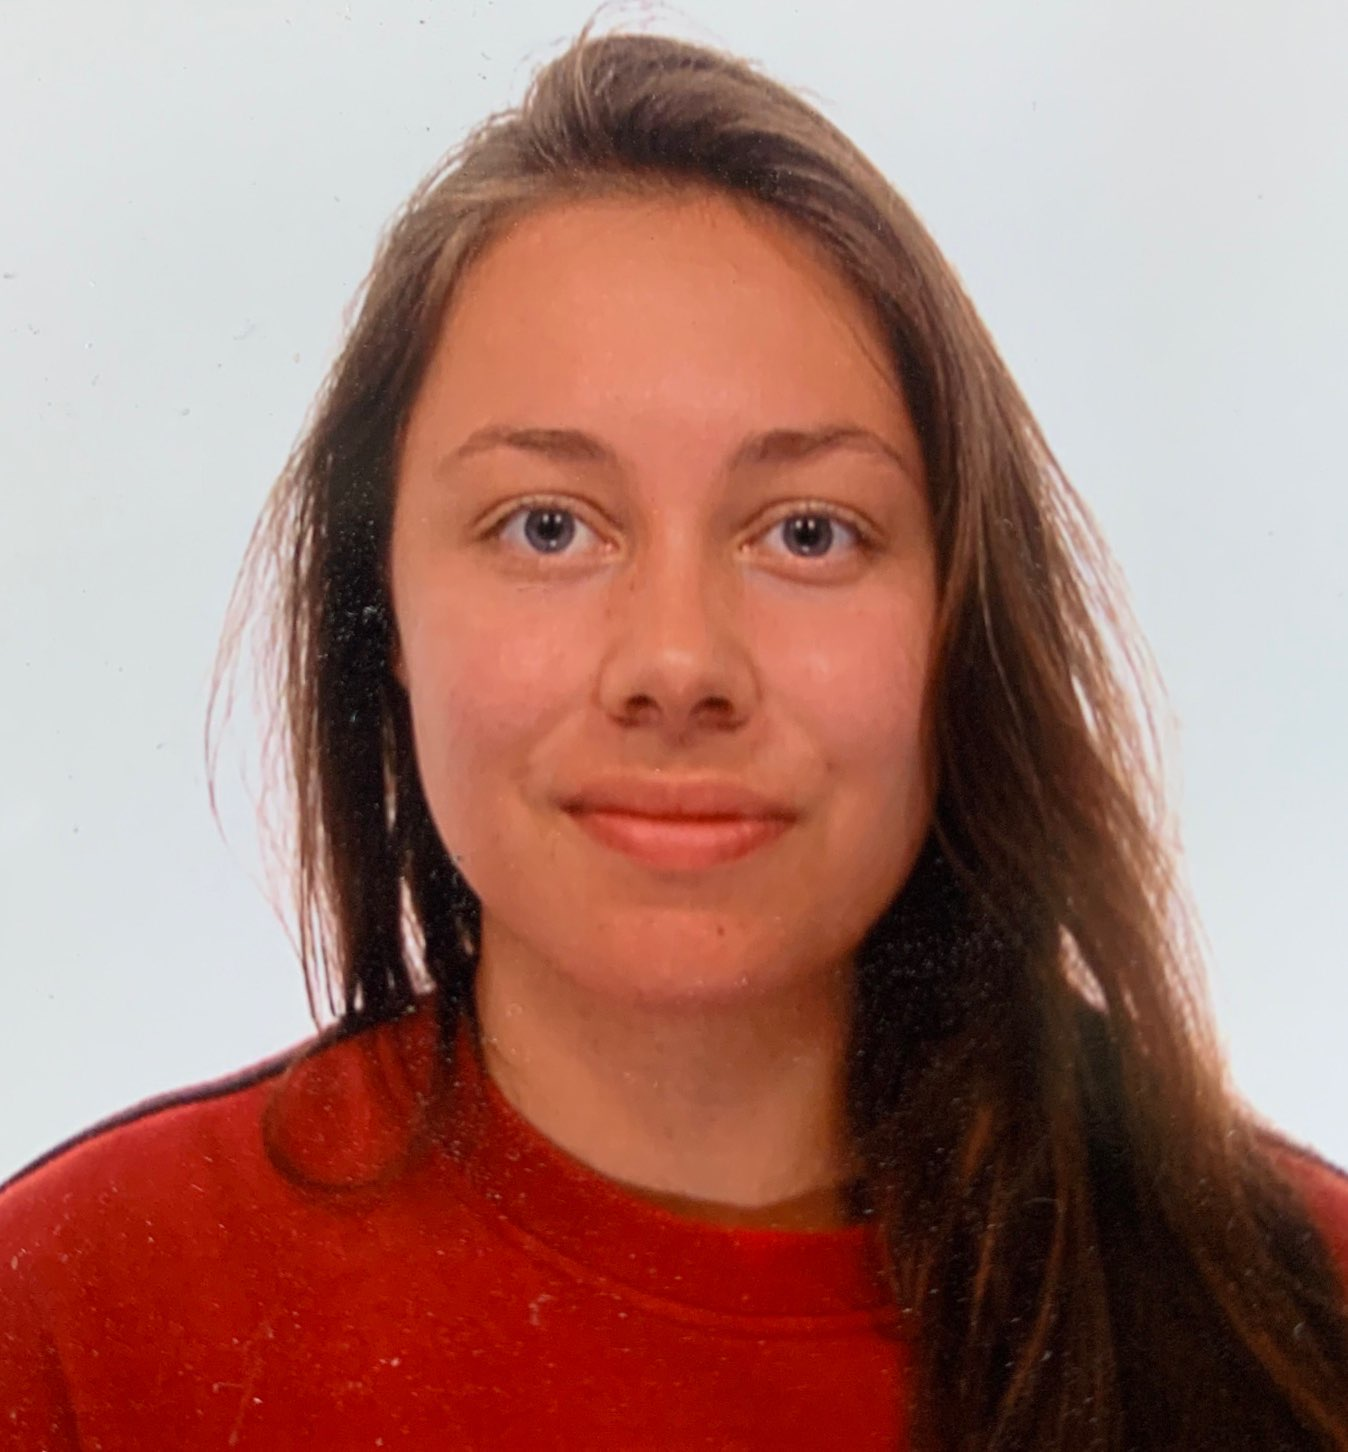
\includegraphics[width=3cm]{profile.jpg}
    \end{flushright}
\end{minipage}
\vspace{1em}

%%%%%%%%%%%%%%%%%%%%%%%%%%%%%%%%%%%%%%%%%%%%%%%%% EXPERIENCE
\section{EXPERIENCE}
\begin{content}

    \begin{position}{Research Assistant, Data Science}{May 2024 -- present}{University of Copenhagen, Denmark}{Prof.~Jeanet Bentzen}{}
        \item Contributed to the {\href{https://www.economics.ku.dk/research/externally-funded-research_new/shocking-religion/}{Shocking Religion}} project on religion's economic impact.
        \item Built topic models to uncover thematic trends in text data.
        \item Created RAG-based LLM pipelines for document insights.
        \item Designed and containerized scalable data workflows; Handled large-scale data ingestion and preprocessing; Deployed solutions on cloud infrastructure (UCloud).
        \item Coordinated with a multidisciplinary research team.
    \end{position}
    
    \begin{position}{Data Scientist}{October 2023 -- May 2024}{Above Sports, Denmark}{}{}
        \item Automated data workflows to improve efficiency.
        \item Developed CV models for brand logo detection.
        \item Worked with product teams to refine output quality.
        \item Dockerized solutions for scalable and reproductible data workflows.
    \end{position}
    
    \begin{position}{Marketing Strategist}{September 2021 -- May 2022}{Crescendo Collective, United States}{}{}
        \item Analyzed campaign data via Google Analytics; Managed Google Ads reporting and strategy.
        \item Automated internal reporting with Python scripts.
        \item Conducted competitor analysis and benchmarks.
        \item Collaborated with data team for audience insights; Presented reports to stakeholders and clients.
    \end{position}
    

\end{content}

%%%%%%%%%%%%%%%%%%%%%%%%%%%%%%%%%%%%%%%%%%%%%%%%% EDUCATION 
\section{EDUCATION} 
\begin{content}
    {\bf M.Sc. Social Data Science} \hfill {\bf 2022 -- 2024} \\
    University of Copenhagen, Denmark \\
    {\bf \em Thesis:} {\href{https://carobs9.github.io/segregation-mobility/}{Mobility and income segregation in Madrid, Spain.}} \\ 
    {\em Elective Courses:} \\
    {\small
    Advanced Machine Learning for Data Science (IT University of Copenhagen) \\ 
    Geospatial Data Science (IT University of Copenhagen) \\
    Advanced Network Science (IT University of Copenhagen) \\
    Natural Language Processing (Department of Computer Science, DIKU) \\
    }

    %\medskip

    {\bf B.Sc. Marketing, Computer Science Minor} \hfill {\bf 2018 -- 2022} \\
    Cardinal Stritch University, United States \\
    %{\em Dean's List (2018--2022)} \\
    {\em Honours:} Dean's List (2018--2022), Best Graduating GPA of Marketing B.Sc. (2022)
\end{content}

%%%%%%%%%%%%%%%%%%%%%%%%%%%%%%%%%%%%%%%%%%%%%%%%% LANGUAGES 
\section{LANGUAGES} 
\begin{content}
    {\bf Spanish:} Native \\
    {\bf English:} Professional Proficiency  \\
    {\bf Galician:} Native \\
    {\bf Portuguese:} Beginner \\
\end{content}

%%%%%%%%%%%%%%%%%%%%%%%%%%%%%%%%%%%%%%%%%%%%%%%%% SKILLS 
\section{SKILLS} 
\begin{content}
    {\bf Programming:} Python {\footnotesize (numpy, tensorflow, matplotlib, pytorch)}, SQL, Bash \\
    {\bf ML \& NLP:} Transformers, Topic Modeling {\footnotesize (umap, hdbscan, bertopic)}, Scikit-learn, Hugging Face \\
    {\bf Geospatial:} Geopandas, Rasterio, QGIS \\
    {\bf Cloud / Tools:} UCloud, Git, Docker, Linux, VSCode
\end{content}

%%%%%%%%%%%%%%%%%%%%%%%%%%%%%%%%%%%%%%%%%%%%%%%%% AWARDS
\section{AWARDS}
\begin{content}
    \prize{Dean's List}{2018--2022}{Achieved Dean’s List every semester of B.Sc. for a GPA above 3.5 with at least 12 credits.} \\
    \prize{Best Graduating GPA of Marketing B.Sc.}{2022}{Graduated with the highest GPA in Marketing of class 2022.} \\
    \prize{Academic and Athletic Grant}{2018--2022}{Received a full scholarship for academic excellence and soccer performance over four years.}
\end{content}

%%%%%%%%%%%%%%%%%%%%%%%%%%%%%%%%%%%%%%%%%%%%%%%%% OPTIONAL: PROJECTS
% Uncomment and fill in if you have real projects to showcase
% \section{PROJECTS}
% \begin{content}
%     \begin{project}{Project Title}{Date}
%         \item Describe the project and your contribution.
%     \end{project}
% \end{content}

\end{document}
